% Template article for document class `jicspack'
% 2004/10/07


\documentclass[print]{jicspack}
\setvolume{11}                             %for printing use only
\setyear{2015}                             %for printing use only
\setpagerange{1}{8}                    %for printing use only
\setheadauthor{X. Liu et al.}          %for printing use only
\setissn{1553--9105} \setpubdate{January 2015} \setno{1}

\afterpage{\beginheader}                   %for printing use only


\usepackage{enumerate}
% if you use PostScript figures in your article
% you can use the graphics package
% \usepackage{graphics}
% or use the graphicx package for more complicated function
\usepackage{graphicx}
% or use the epsfig package
% \usepackage{epsfig}

% The amssymb package provides various useful mathematical symbols
\usepackage{amssymb}

\begin{document}

\begin{premaker}

% The premaker environment contains Title, authors and addresses;
% use the thanksref command within \title, \author or \address for footnotes;
% use the corauthref command within \author for corresponding author footnotes;
% use the ead command for the email address,
% and the form \ead[url] for the home page:
% \title{Title\thanksref{label1}}
% \thanks[label1]{}
% \author{Name\corauthref{cor1}\thanksref{label2}}
% \ead{email address}
% \ead[url]{home page}
% \thanks[label2]{}
% \corauth[cor1]{Corresponding author}
% \address{Address\thanksref{label3}}
% \thanks[label3]{}

\title{An Improved Imputation Method for Missing Data Based on QENNI \thanksref{label1}}
\thanks[label1]{Project supported by the National Nature Science Foundation of China (No. ***).}
\author[author1]{Zhaoyu Zhang\corauthref{cor1}},
\ead{china.zhangzhaoyu@gmail.com}
%\thanks[label2]{Footnotes for authors}
\corauth[cor1]{Corresponding author.}
% other authors
\author[author2]{Zhibo Chen},
\author[author3]{JianXin Wang}

\address[author1]{School of Information Science And Technology, Beijing Forestry University, Beijing 100083, China}
\address[author2]{School of Information Science And Technology, Beijing Forestry University, Beijing 100083, China}
\address[author3]{School of Information Science And Technology, Beijing Forestry University, Beijing 100083, China}
%\thanks[label3]{Footnotes for address}
% you can use optional labels to link authors explicitly to addresses:
% \author[label1]{},
% \author[label2]{}
% \address[label1]{}
% \address[label2]{}

\begin{abstract}
% Text of abstract
Missing data imputation is an important research aspect in data mining. Data quality is a major concern in Machine Learning and other correlated areas such as Knowledge Discovery from Databases (KDD). Many imputation methods of missing data have been designed to resolve the problem. More or less, they have some deficiencies. As the K-Nearst Neighbor Imputation (KNNI) algorithm is often biased in choosing the $k$ mearest neighbors of missing data. A new imputation method is put forward, Quadrant Encapsidated Nearest Neighbor based Imputation method (QENNI). QENNI uses the quadrant nearest neighbors around a missing datum to impute the missing datum. It is not biased in selecting nearest neighbors. Experiments demonstrate that QENNI is much better than the kNNI method in imputed accuracy. But, as the experiment proceeded, we found out the denseness of points in each quadrant and the distance between the two point affect the missing data value badly. So, we improved the QENNI algorithm and put forward Denseness and Distence Weighted Quadrant Encapsidated Nearest Neighbor based Imputation method algorithm (DDWQENNI). The experimental result demonstrates that our DDWQENNI method has a higer imputation accuracy than QENNI.
\end{abstract}
\begin{keyword}
% keywords here, in the form: keyword \sep keyword
Imputation of missing data \sep Quadrant  \sep KNNi \sep QENNI \sep WQENNI
\end{keyword}
\end{premaker}

% main text
\section{Introduction}
\label{Maintext}
Data mining \cite{NumeApp} is an interdisciplinary subfied of computer science. It is the computational process of dicovering patterns in large data sets involving methods at the intersection of artificial intelligence, machine learning, statistics, and database systems. The overall goal of the data mining process is to extract information from a data set and transform it into an understandable structure for further use. Data mining is a powerful technology with great potential. Pre-processing as one of the indispensable step of data mining can seriously affect the accuracy of the conclusion. That is why missing data imputation has been an inevitably and challenging research.

Due to its importance in Dataing mining, missing data imputation has received considerable attention during the past decades. A large percentage of studies have been done to develop procedures to deal with missing values. Recently, no matter in which filed of study, $kNNI$ \cite{NumeApp} imputation method has been researched and applied widely because of its easy operating, high efficiency an accuracy. It is an excellent imputation algorithm, but thoes choosing nearest neighbors of misssing data is very likely biased in one side. So it's not the best choice to use them for missing data imputation. In addiction, the parameter $k$ is the key factor for the $kNNI$ algorithm. In the experiments, if the $k$ sets a larger value, it brings seriously randomness; if the $k$ sets a smaller value, it will lose large sample size standard of statistics. Before very experiment of $kNNI$, lots of calculation should be token to get the approproate vlaue of $k$. It makes the algorithm more complex. In response to these prolems, Shichao zhang \cite{NumeApp} put forward a new missing data imputation algorithm, quadrant encapsidated nearest neighbor based imputation ($QENNI$). QENNI algorithm imputes the missing data by finding all of the quadrant encapsidated nearest neighbors of the missing data.Exactly to say, it assumes the missing data as the center, the complete data sets are distributed to each quadrant. Because of this feature, it can void the heavily depending on the parameter $k$ of kNNI. Experimental results show QENNI has a higer accuracy than kNNI.

But, according to the analysis of the missing data, we find it also seriously affected by denseness of points in each quadrant and the distance between the missing data and complete data. So, based on QENNI,  we take the denseness and distance's weight into account and proposes a new missing data imputation, Denseness and Distence Weighted Encapsidated Nearest Neighbor based Imputation method ($DDWQENNI$). This imputation algorithm overcomes the above-mentioned limitations and has a good performance than QENNI.

The rest of this paper is organized as follows: Section 2 introduces the details of the proposed imputation method and give the corresponding algorithm. Seciont 3 gives the experiments and results. Section 4 discusses the result and drwas a conclusion.

\section{DDWQENNI Algorithm}
\label{sec:2.1}
On the basis of the above discussion, in this part, we give the defination and implementation of the DDWQENNI algorithm. The improvement of DDWQENNI algorithm will be pointed out. We also discuss the shortcomings of kNNI and QENNI.
\subsection{Algorthm background}
Suppose $X$ is an M-dimensional random vector, $Y$ is the dependent variable affected by $X$. In practice, if a missing data random sample (size is $n$) can be get, it can be expressed as $(X_i, Y_i, \delta_i), i= 1, 2,\cdots, n$. In which, all of the $X_i$ vector is observable, when $Y_i$ is missing, $\delta_i = 1$, otherwise $\delta_i = 0$. If the data set $T$ contains $n$ data, each data has $m + 1$ attributes (contains $m$ condition attributes and $1$ decision attribute), keep: $T_i = (X_{i1}, X_{i2}, \cdots, X_{im}, Y)$ (missing values are generated only in decsion attribute $Y$). $T = I \bigcap C$, let $r = \sum\limits_{k=1}\limits^{n} \delta_i$, $I = {T_1, \cdots, T_r}, r \leq n$ are the data sets which decision attrubutes are missing, referred to missing data sets; $C = {T_r+_1, \cdots, T_n}$ are the complete data sets.
\subsection{$k$NNI algorithm}
\label{2.2}
K-Nearst Neighbor Imputation ($k$NNI) imputes the missing value by the $k$ nearest neighbors of the missing data. It bases on the theory that the closer the distance, the closer the relation. If a data loses one attrubute, to find out the $k$ nearest neighbors in complete data sets and use the average value of them to impute the missing value.

As previously mentioned, $k$NNI is praised by the majority of researchers because of its simple operation, low time complexity and high imputation accuracy. But there are still some drawbacks. The $k$ nearest neighbors selected by $k$NNI algorithm may occur preferences, which makes the filling effect is relatively inefficient. In fact, from the distribution of complete data which surrounds the missing data, the distribution of its nearest neighbors data and overall data may be inconsisten. For instance, as shown in Fig.\ref{fig:figure1}, $O$ represents missing data, the other points represents complete data, we use $k$NNI algorithm to impute the missingd data value. According to the 2.2, we need to find three nearest neighbors and use them to impute the missing data value. So $A, B, C$ are selected. Nevertheless, from Fig.\ref{fig:figure1} we can clearly see that the complete data surrouding the missing data are evenly distributed, but the three selected nearest neighbors bias in the first quadrant. So the three nearest neighbors may not be the best choice and may not be able to get the best results by using them to impute the missing value.

\begin{figure}[h]
\centering
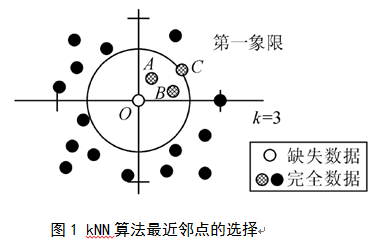
\includegraphics[angle=0, width=0.5\textwidth]{figure1.png}
\caption{Nearest neighbors chosen by $k$NN}
\label{fig:figure1}
\end{figure}

To choose the $k$ parameter of $k$NNI algorithm is diffuclt. Each time, we use $k$NNI to impute the missing data, we need to repeat the experiment so many times to obtain the value $k$. Once the value of $k$ occurs deviation, the performance of $k$NNI will be significantly lower. In conclusion, if the algorithm can eliminate the dependence on the parameter $k$, it will be the best choice.

\subsection{QENNI algorithm}
\label{2.3}
We propose the hypothesis that the complete data which is used to impute missing data must be the nearest neighbors and in the first encirclement of the missingd data. we also need to eliminate the dependence on the parameter $k$. Let's realize the idea below.

\begin{figure}[h]
\centering
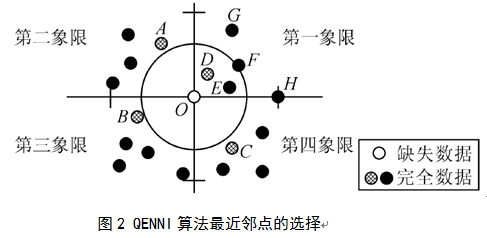
\includegraphics[angle=0, width=0.5\textwidth]{figure2.png}
\caption{Nearest neighbors chosen by QENNI}
\label{fig:figure2}
\end{figure}

\begin{enumerate}[(1)]
\item First, take data $(X_i, X2, \cdots, X_m)$ which contains $m$ condition attributes as a point of $m$-dimensional space, estabish a coordinate system and the missding data is the center. Through the axis to divide the $m$-dimensional into $2^m$ quadrants.
  \begin{enumerate}[a.]
  \item When $m = 2$, the condition attributes $(X_1, X_2)$ can be regard as a point of plane. As shown in Fig.\ref{fig:figure2}, the axis divides the plane into $2^2$ quadrants. If one point is just between the two quadrants, we classify it to one of its nearby quadrant. According to our difinition, everyone of the data set can be located on the only certainty quadrant.
  \item Similarly,when $m = 3$, the condition attributes of data is $(X_1, X_2, X3)$. The Formed spatial coordinate system divides the space into $2^3$ quadrants and everyone of the data is also in the only identified quadrant.
  \item Extended to the general case, when $m = m$, the condition attributes of data is $(X_i, X2, \cdots, X_m)$ and the space is divided into $2^m$ quadrants.
  \end{enumerate}
\item Based on the dividing of $m$-dimensional space, the Euclidean distance of each point from its own to the center (which is the missing data) is calculated. To find out the nearest one of each quadrant (if not exists, ignore it) and use decision attributes of them to impute the missing data value. With $m = 2$, for example, as shown in Fig.\ref{fig:figure2}. In each quadrant,  we select $A, B, C, D$ as the nearest neighbors and use the decision attributes $Y$ of them to impute the missing data value of center $O$. It also weighted by the distance of each selected point. Obviously, the way of QENNI to choose the nearest neighbors is different from the $k$NNI algorithm.
\begin{equation}
\label{eq:1}
dist(T_i, T_j) =\sqrt{ \sum\limits_{k=1}\limits^{m} (X_{ik} - X_{jk})^2}
\end{equation}
\item In order to analyze the effectiveness of the algorithm better, for each missing data $T_i (T_i \in I)$, on the basis of QENNI algorithm,  the following definition can be given:
\begin{description}
\item[Step 1] The coordinate system centered at $T_i$ divides the space into $2^m$ quadrants and the complete data set $C$ based on quadrant is divided into $2^m$ subset $C = \{D_1, D_2, \cdots, D_q, \cdots, D_{2^m}\}$. Each complete data set $D_q (q = 1, 2, \cdots, 2^m)$ is the $q$ quadrant's data of $T_i$.
\item[Step 2] $\forall T_j \in D_q$, satisfy $Near_q = \arg \min dist_{T_j \in D_q}(T_i, T_j)$, $Near_q$ is nearest neighbor of $T_i$ in $q$ quadrant. As shown in Fig.\ref{fig:figure2}, the first quadrant data of $T_o$ is $D_1 = \{T_D, T_E, T_F, T_G, T_H \}$. So $Near_q = T_D$ which is the nearest neighbor of first quadrant.
\item[Step 3] In the $q$ quadrant, take $T_i$ as the center of the sphere (or hypersphere), dist($Near_q, T_i$) as the radius to ensure the $Shell_q$ of $T_i$ in $q$ quadrant.
\item[Step 4] All of the $Shell_q (q = 1, 2, \cdots, 2^m)$ and axis constitute the $m$-dimensional subspace which is Shell of $T_i$.
\item[Step 5] All the of nearest neighbor $\{Near_1, Near_2, \cdots, Near_{2^m}\}$ of $T_i$ in every quadrant are called the points of Shell.
\item[Nature 1] If $D_q \neq \O$, the Shell of $T_i$ must exist in $q$ quadrant.
\item[Nature 2] $\forall T_j \in D_q$, $\exists dist(T_j, T_i) \geq dist(Near_q, T_i)$.
\end{description}
\item In summary, the QENNI algorithm can overcome the shortcomings of $k$NNI in choosing the $k$ nearest neighbors of missing data. The selected complete data is not biased in any side and the Shell of the missing data is smallest. That is to say it does not exist any other complete data on the Shell of the missing data. It is thus clear that QENNI algorithm can find out the most satisfied complete data without any preferences. They can represent the missing data better than $k$NNI.
\end{enumerate}

\subsection{DDWQENNI aglorithm}
\label{2.4}
Even though the QENNI algorithm has a better performace than $k$NNI, it does not take the denseness into account. As shown in Fig.\ref{fig:figure3}, if we just think about the distance of complete data $A$ and $D$, the $A$ has a higher affect of the result. But it is clear that just the distance can not represents the real affect of the complete data $A$. If the denseness of complete data which surrounds $A$ is token into accout, it may have a higer weight than $D$. Based on the above considerations, Our new algorithm takes both the weight of distance and denseness into accout. The fellowing definitions are given.
\begin{figure}[h]
\centering
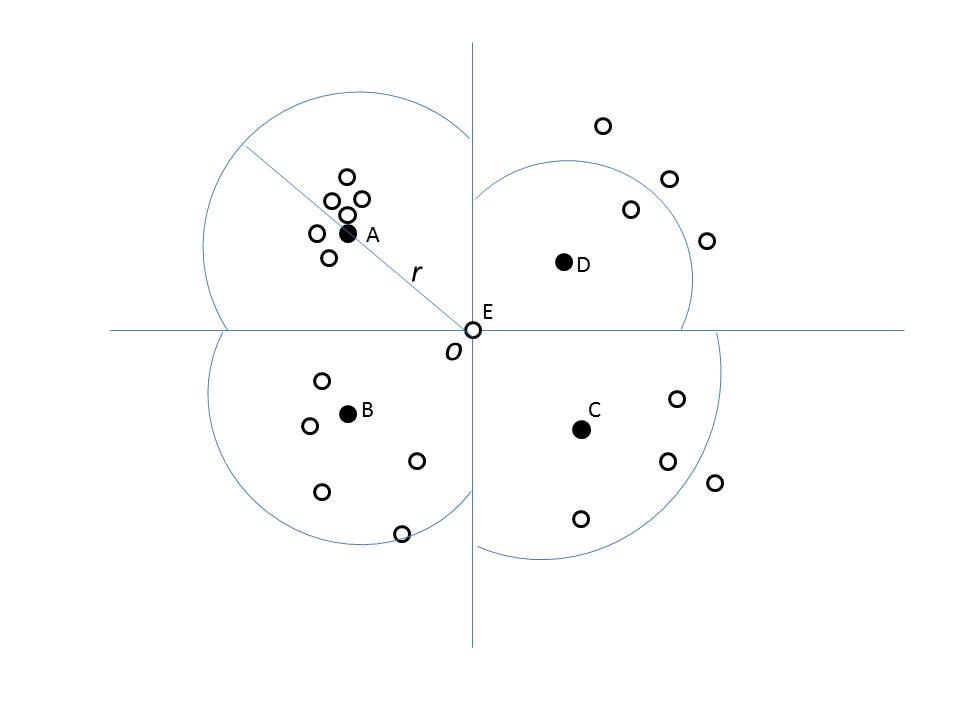
\includegraphics[angle=0, width=0.6\textwidth]{figure3.jpg}
\caption{Nearest neighbors chosen affected by Denseness}
\label{fig:figure3}
\end{figure}

\begin{enumerate}[(1)]
\item Weight of Distance : The different length of distance has differnet size of influence. The more closer, the higher wieght. So we keep weight of each nearest neighbor $Near_i (i=1, 2, \cdots, 2^m)$ in every quadrant as:
\begin{equation}
\label{eq:2}
W(D)_i = \frac{1}{dist(Near_i, T_i)^2}
\end{equation}
\item Weight of Denseness : The denseness represents the number of complete data in per unit volume and it can indicate the wight of the quadrant's denseness. We use Eq. (\ref{eq:3}) to calculate the volume of n-sphere. The Eq. (\ref{eq:5}) is used to calculate the denseness which can represents the weight. Each quadrant's number complete data is counted as $N = \{N_1, \cdots, N_i, \cdots, N_{2^m}\}$.

\begin{equation}
\label{eq:3}
V_n(R) = \frac{\pi^{\frac{n}{2}}R^n}{\Gamma (\frac{n}{2} + 1)}
\end{equation}

\begin{eqnarray}\label{eq:4}
\Gamma(\frac{n}{2} + 1) = \left\{\begin{array}{ll}(\frac{n}{2})! & \mbox{n is Even} ,\\\sqrt{\pi}\frac{n!!}{2^{\frac{n+1}{2}}} & \mbox{n is Odd}.\end{array}\right.
\end{eqnarray}

\begin{equation}
\label{eq:5}
W(\rho)_i = \frac{N_i}{\frac{V_n(R)_i}{2^m}}
\end{equation}

\item Core algorithm : The algorithm takes both denseness and distance's weight into consideration and bring in the factor $\beta (0.0 \leq \beta \leq 1.0)$ to decide the percentage of denseness and distance.  The detail steps of DDWQENNI are as follows:
\begin{enumerate}[a.]
  \item Calculate the Euclidean distance of missing data set $I$ and complete data set $C$ by Eq. (\ref{eq:1}).
  \item Iterate data set $I$ and $C$ calculate the nearest neighbor, total number of complete data in each quadrant where $R \leq 2 * dist(Near_i, I_i)$ and volume of each hyperspace by Eq. (\ref{eq:2}, \ref{eq:3}, \ref{eq:5}).
  \item The key about how to figure the complete data for each quadrant is to translate the data vector into a number and use it to mark the quadrant. First, translate the coordinate into a vector consisting of one and zero. if the value of vector greater than zero, translate it into one, otherwise keep it as zero. Than, translate the binary number into decimal.
  \begin{equation}
  \label{eq:6}
  \begin{pmatrix} 2& -1& 0\end{pmatrix}\Rightarrow \begin{pmatrix} 1& 0& 0\end{pmatrix} \Rightarrow (1*2^2 + 0*2^1+ 0*2^0) \Rightarrow 4
  \end{equation}
  \item Take the previous results into Eq. (\ref{eq:7}) to calculate the missing data value ($v_i$). The equation has token theweight of denseness and distance into account.
  \begin{equation}
  \label{eq:7}
  v_i = \frac{\sum\limits_{i=1}\limits^{n}((1-\beta)W(D)_i + \beta W(\rho)_i) * D_i}{\sum\limits_{i=1}\limits^{n}((1-\beta)W(D)_i + \beta W(\rho)_i}
  \end{equation}
\end{enumerate}
\end{enumerate}

\section{Experiments and Results}
\subsection{Dataset}
\label{sec:1.1}
In order to test our Algorithm, we choose the open dataset Abalone which is from UCI and Delta\_ailerons which is from weka. We do the same experiments as QENNI does. The sex attribute is excluded and left the data whoes sex value is $M$. It has 8 attribute and 1528 records in total. The Diameter attribute is chosen as decision attribute and missing data is generate on it. The Delta\_ailerons dataset has 6 attributes and 7129 records in total. The last attribute is chosen as descsion attribute and the missing data is generated on it. The imputation accuracy is used as evaluation index. In general, the Root Mean Square Error (RMSE) is used. $e_i$ is the original value, $e'_i$ is the imputation value and $m$ is the number of missing data. The smaller the RMSE, the higer the imputation accuracy.
\begin{equation}
\label{eq:6}
RMSE = \frac{1}{m}\sum\limits_{1=1}\limits^{m}(e_i - e'_i)^2
\end{equation}

\subsection{Experiments}

\subsection{Results analysis}


\section{Conclusion}
For improving the efficiency and accuracy of missing data imputaion, DDWQENNI imputation algorithm has been put forward. The method is able to overcome the limitations of kNNI and QENNI. The innovation of our method is to take the denseness of points in each quadrant and distence between the compelte data and the missing data into consideration. So, the imputed data can be more closer to the missing data. The experimental results indicate that DDWQENNI algorithm has a better performance than QENNI. Feature work is to improve the computing speed of WQENNI in hyperspace.

\section{Introduction}
\label{Maintext}
\begin{itemize}
\item{\bf Common} Contributions must be written in English. Each
paper should be introduced by a list of keywords and a
self-contained abstract of no more than thirty lines without long
formulas. \item{\bf Title} Title should be concise but
informative. Titles are often used in information-retrieval
systems. Avoid abbreviations and formulae where possible.
\item{\bf Author} There should be and should only be one
corresponding author. \item{\bf Abstract} A concise and factual
abstract, of aro und 100 words, is required. The abstract should
state briefly the purpose of the research, the principal results
and major conclusions. It must be able to stand alone, references
should be avoided. Non-standard or uncommon abbreviations should
be avoided. \item{\bf Keywords} Three to five keywords are
required, using British spelling and avoiding general and plural
terms and multiple concepts (avoid, for example, ``and", ``of").
\item{\bf Headings} Papers should be divided into numbered
sections, subsections and, if necessary, subsubsections (e.g. 3,
3.1, 3.1.1, etc.). \item{\bf Uppercase \& Lowercase} Every word
within the title of ``section" , except empty word, should has its
initial capitalized. But for the ``subsection" , the only word
that should be capitalized is the first one. But note that it is
not the case for subsection, see subsection
\ref{subsectiontitlerule}. \item{\bf Mathematical Symbols} Every
mathematical symbol in the text, for example, $n, R, x, y$ etc.
\item{\bf Enumerations} Enumerations should be listed in an
Item-like environment, e.g. ``itemize" ``enumerate". \item{\bf
Footnotes} Footnotes should be avoided if possible and as brief as
possible, they should be numbered consecutively. \item{\bf
Algorithms} If you are presenting an algorithm or listing
something with order, make sure you use the ``itemize" or
``enumerate"  environment, treat each step as an ``item" and label
it as ``($n$)", where $n$ is the sequence number of steps. For the
sub-items label them as ``a.", ``b." , etc., see section
\ref{sec:1.1}. \item{\bf Figures} Figures should be numbered
consecutively in the order of appearance and citation in the text.
Be sure to cite every figure. Handwritten lettering and
low-quality computer graphics are not acceptable. EPS electronic
files should be sized as they will appear in the journal.
\item{\bf Tables} Tables must be numbered and typed on separate
pages. The table title, which should be brief, goes above the
table. Detailed explanations or table footnotes should be typed
directly beneath the table. Note that tables are usually typeset,
not scanned (tables cannot be electronically reduced in size).
\item{\bf Citations} Citations should coupled with labels. That
is, to make a citation , you should label the position first, then
use the command ``\verb|\ref|". All citations made in this guide,
including equations, tables, figures, etc., follow this rule, you
can check the source file to make a clearer understood. \item{\bf
References} References must be numbered consecutively in the order
of their first citation, as in the following examples: books
\cite{NumeApp,texbook}, articles in journals \cite{UncaliEu},
papers in a contributed volume \cite{Deformation,canonical},
unpublished papers \cite{SpaceDeform}.
\end{itemize}
\subsection{Only the first word in the title of ``subsection" be capitalized}
\label{sec:1.1}
We place a paradigm for the algorithm here:
\begin{enumerate}[(1)]
\item The first step.
\item The second step.
  \begin{enumerate}[a.]
  \item substep1.
  \item substep2.
  \end{enumerate}
\item  The last step.
\end{enumerate}
In the ``.tex" file it may look like the following:
\begin{verbatim}
\begin{enumerate}[(1)]
\item The first step.
\item The second step.
  \begin{enumerate}[a.]
  \item substep1.
  \item substep2.
  \end{enumerate}
\item  The last step.
\end{enumerate}
\end{verbatim}

You can also use description environment, for example
\begin{description}
\item[Step 1] The first step. \item[Step 2] The second step.
\item[Step 3] The second Step.
\end{description}
In the ``.tex" file it may look like the following:
\begin{verbatim}
\item[Step 1] The first step.
\item[Step 2] The second step.
\item[Step 3] The second Step.
\end{verbatim}
{\bf Note:} Package ``enumerate" is needed for this kind of usage
of environment of enumerate. \label{subsectiontitlerule}
\section{Mathematical Notation}
\subsection{Build-in environments}
This document class has provided you some commonly used environments:
\begin{itemize}
\item{Definition environment}\\
{\verb|\begin{defn}|
$\cdots\cdots$
\verb|\end{defn}|}
\item{Lemma environment}\\
{\verb|\begin{lem}|
$\cdots\cdots$
\verb|\end{lem}|}
\item{Theorem environment}\\
{\verb|\begin{thm}|
$\cdots\cdots$
\verb|\end{thm}|}
\item{Proof environment}\\
{\verb|\begin{pf*}{Proof}|
$\cdots\cdots$ \verb|\end{pf*}|}
\item{Corollary environment}\\
{\verb|\begin{col}|
$\cdots\cdots$
\verb|\end{col}|}
\item{Proposition environment}\\
{\verb|\begin{pro}|
$\cdots\cdots$
\verb|\end{pro}|}
\end{itemize}

The following examples demonstrate the usage of the above environments.
\begin{defn}
A graph $G$ is an ordered pair of disjoint sets $(V,E)$ such that $E$ is a subset of the set
of unordered pairs of $V$.
\end{defn}
\begin{lem}
If $m\geqslant 2n$ then $\epsilon(\overrightarrow{G};x,y)=0$.
\end{lem}


\begin{thm}
A graph is bipartite if it does not contain an odd cycle.
\end{thm}
\begin{pf*}{Proof}
Suppose $G$ is bipartite with vertex classes $V_1$ and $V_2$.
Let $x_1x_2\cdots x_l$ be a cycle in $G$.
We may assume that $x_1\in V_1$. Then $x_2\in V_2$, $x_3\in V_1$,and so on:
$x_i\in V_1$ if $i$ is odd.
Since $x_l\in V_2$, we find that $l$ is even.\\
\indent{}Suppose now that $G$ does not contain an odd cycle. Since a graph is bipartite if each component of it is,
we may assume that $G$ is connected. Pick a vertex $x\in V(G)$ and put $V_1=\{y| d(x,y)\mbox{is odd}\}$,
$V_2=V\backslash V$. There is no edge joining two vertices of the same class $V_i$ since otherwise $G$ would contain an odd cycle.
Hence $G$ is bipartite.
\end{pf*}
\begin{thm}
A graph is a forest if for every pair $\{x,y\}$ of distinct vertices it contains at most one $x$-$y$ path.
\end{thm}
\begin{pf*}{Proof}
If $x_1x_2\cdots x_l$ is a cycle in a graph $G$ then $x_1x_2\cdots x_l$ and $x_1x_l$ are two $x_1$-$x_l$ paths in $G$.\\
\indent{}Conversely, let $P_1=x_0x_1\cdots x_l$ and
$P_2=x_0y_1y_2\cdots y_kx_l$be two distinct $x_0$-$x_l$ paths in a
graph $G$. Let $i+1$ be the minimal index for which $x_{i+1}\neq
y_{i+1}$, and let $j$ be the minimal index for which $j\geqslant
i$ and $y_{j+1}$ is a vertex of $P_1$, say $y_{j+1}=x_h$. Then
$x_ix_{i+1}\cdots x_ky_jy_{j-1}\cdots y_{i+1}$ is a cycle in $G$.
\end{pf*}
\begin{col}
Every connected graph contains a spanning tree, that is a tree containing every vertex of the graph.
\end{col}
\begin{pf*}{Proof}
Take a minimal connected spanning subgraph.
\end{pf*}
\begin{col}
A tree of order $n$ has size $n-1$; a forest of order $n$ with $k$ components has size $n-k$.
\end{col}
\begin{defn}
An oriented graph is a directed graph obtained by orienting the edges,
that is by giving the edge $ab$ a direction $\overrightarrow{ab}$ or $\overrightarrow{ba}$.
Thus an oriented graph is a directed graph in which at most one of $\overrightarrow{ab}$ and $\overrightarrow{ba}$ occurs.
\end{defn}
\begin{pro}
The set
$$S_m^\mu(\Delta)=\{f|\  {\rm deg} f\leqslant m, f\in S_m^\mu(\Delta)\}$$
is a finite-dimensional linear vector space on $k$, $m\geqslant
0$.
\end{pro}
\begin{lem}
$G$ is Hamiltonian if $C_n(G)$is and $G$ has a Hamilton path if so does $C_{n-1}(G)$.
\end{lem}
{\bf Note:} If you use the above environments, it will be numbered
automatically. If the above environments failed to prove their
sufficiency, feel free to define your own theorem-like
environments, i.e. \verb|\newtheorem\{Name\}\{Caption\}|.
%Make sure that all of your arrays display in the displaystyle.
\subsection{Equations}
\label{equsection}
%We recommend that you follow the following rules to make your article more readable and intelligible.
%Lengthy equations should be placed in the Mathematical environment, i.e. \verb|$$ $$| or \verb|\begin\{math\}| $\cdots$ \verb|\end\{math\}|.
Here are some examples of equations that cover the rules of making a equation with explanations following.

Expressions that are too long or oversized should be separated
from the main text, i.e. be surrounded by
\verb|$$|$\cdots$\verb|$$|. For example,
$$
f(x)=\sum\limits_{k=1}\limits^{\infty}c_kT_{3^k}(x).$$

Never try to number the equation manually. If you want to number a
equation, use the corresponding environment, i.e. \verb|Equation|
or \verb|Eqnarray| if you want to display mutiple equations with
numbers. Eq. (\ref{eq:1}, \ref{eq:2})  and Eq. (\ref{eq:3})
demonstrate the usage of \verb|Equation| and \verb|Eqnarray|
environments respectively.
\begin{equation}\label{eq:1}
p(x)=a_0+a_1+\cdots+a_nx^n.
\end{equation}
\begin{equation}\label{eq:2}
[L/M]=\frac
{\left|
\begin{array}{cccc}
a_{L-M+1} & a_{L-M+2} & \cdots & a_{L+1}\\
\vdots & \vdots &  & \vdots\\
a_{L} & a_{L+1} & \cdots & a_{L+M}\\
\sum\limits_{j=M}\limits^{L}a_{j-M}{X^j} & \sum\limits_{j=M-1}\limits^{L}a_{j-M+1}{X^j} & \cdots & \sum\limits_{j=0}\limits^{L}a_{j}{X^j}\end{array}
\right|}
{\left|
\begin{array}{cccc}
a_{L-M+1} & a_{L-M+2} & \cdots & a_{L+1}\\
\vdots & \vdots &  & \vdots\\
a_{L} & a_{L+1} & \cdots & a_{L+M}\\
x^{M} & x^{M-1} & \cdots & 1
\end{array}
\right|}.
\end{equation}
\begin{eqnarray}\label{eq:3}
K_m(t)&=&\frac{1}{(m-1)!}E((x-t)_{+}^{m-1};\alpha)\nonumber\\
      &=&\frac{1}{(m-1)!}\left((\alpha-t)_{+}^{m-1}-\sum\limits_{k=0}\limits^{n}l_k(\alpha)(x_k-t)_{+}^{m-1}\right).
\end{eqnarray}

Use \verb|displaystyle|  to make formulas bigger when necessary.
\begin{equation}\label{eq:4}
f(z)\thickapprox\frac{\displaystyle 1+\frac{1}{2}z+z^2+\frac{1}{2}z^3}{\displaystyle 1-\frac{1}{2}z+z^2}.
\end{equation}

The texts in the equations should not be writing in the
mathematical form, you can use \verb|\mbox{#text}| to achieve
this, example is given in Eq. (\ref{eq:5}).


\begin{eqnarray}\label{eq:5}
f(x)=\left\{\begin{array}{ll}3x^2 & \mbox{when}\ x\geqslant 0,\\-3x^2 & \mbox{when}\ x\leqslant 0.\end{array}\right.
\end{eqnarray}

When dealing with well-known functions like min, sin, cos , etc.,
you should use their normal form in the math environment, i.e. use
\verb|\min, \sin, \cos,| $\cdots$ respectively.
$$\arg\min\{\sin{x}\times\cos(x)\}$$
$$\arg\min\{\sin{x}\times\cos(x)+f(x)-g(x)+e(x)\},$$

If a sentence is not ended at a equation, the words follows the
sentence may not be initial capitalized and intend, see Eq.
(\ref{eq:6}).

 Then the unconditional pdf of $X$ is
\begin{equation}\label{eq:6}
f_X(x)=\int f_{X|\Theta}(x|\theta)f_{\Theta}(\theta)d\theta,
\end{equation}
where the integral is taken over all values of $\theta$ with positive probability.
\section{Table Section}
Use ``Table" or ``Tabular" environment as usual. You may center
the table most of the time to beautify your article. You also
should name each table. Table [\ref{lab:1}, \ref{lab:2}] are two
typical examples of tables.
\begin{table}[h]
\centering \caption{Observation results for LSE} \label{lab:1}
\begin{tabular}{|c|c|c|c|c|c|c|c|c|}
\hline $k$   & 1 & 2 & 3 & 4 & 5 & 6 & 7 & 8\\
\hline $x_k$ & 0 & 1 & 2 & 3 & 4 & 5 & 6 & 7\\
\hline $y_k$ & 1.4 & 1.3 & 1.4 & 1.1 & 1.3 & 1.8 & 1.6 & 2.3\\
\hline
\end{tabular}
\end{table}
\begin{table}[h]
\centering \caption{Primitive types in Java}
\label{lab:2}
\begin{tabular}{|c|c|c|c|c|}
\hline
Primitive type & Size & Minimum & Maximum & Wrapper type\\\hline
boolean & -- & -- & -- & Boolean\\\hline
char & 16-bit & Unicode 0 & Unicode $2^{16}-1$ & Character\\\hline
byte & 8-bit & -128 & +127 & Byte\\\hline
short & 16-bit & $-2^{15}$ & $+2^{15}-1$ & Short\\\hline
int & 32-bit & $-2^{31}$ & $+2^{31}-1$ & Integar\\\hline
long & 64-bit & $-2^{63}$ & $+2^{63}-1$ & Long\\\hline
float & 32-bit & IEEE754 & IEEE754 & Float\\\hline
double & 64-bit & IEEE754 & IEEE754 & Double\\\hline
void & -- & -- & -- & Void\\\hline
\end{tabular}
\end{table}
\section{Figure Section}
\label{Figuresection}
If you have figures, include them like this:
\begin{figure}[h]
\centering
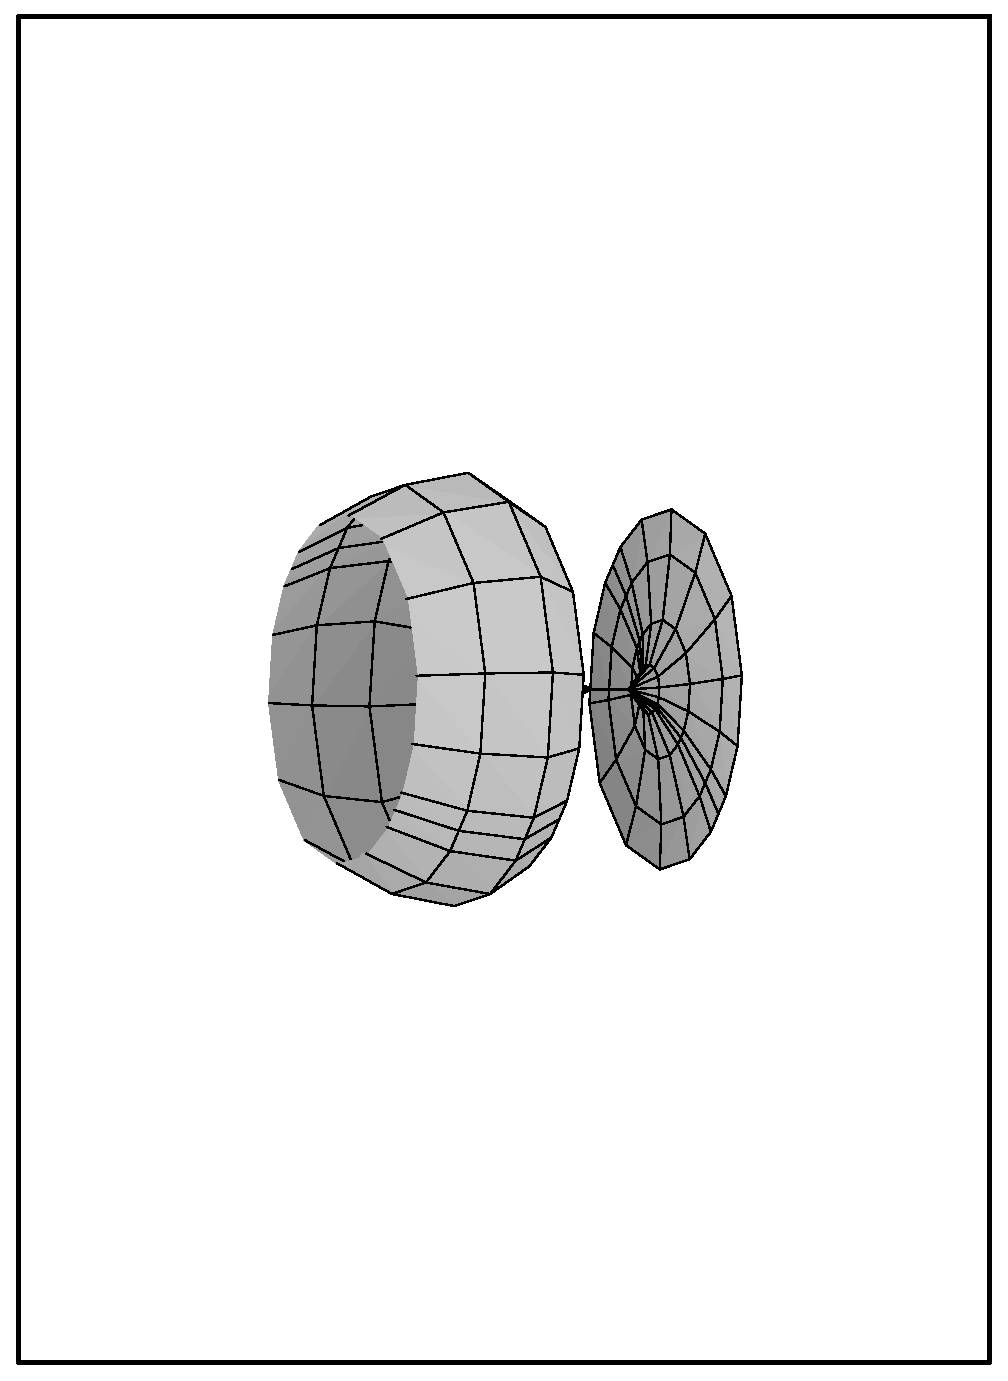
\includegraphics[angle=-90, width=0.3\textwidth]{cup1.eps}
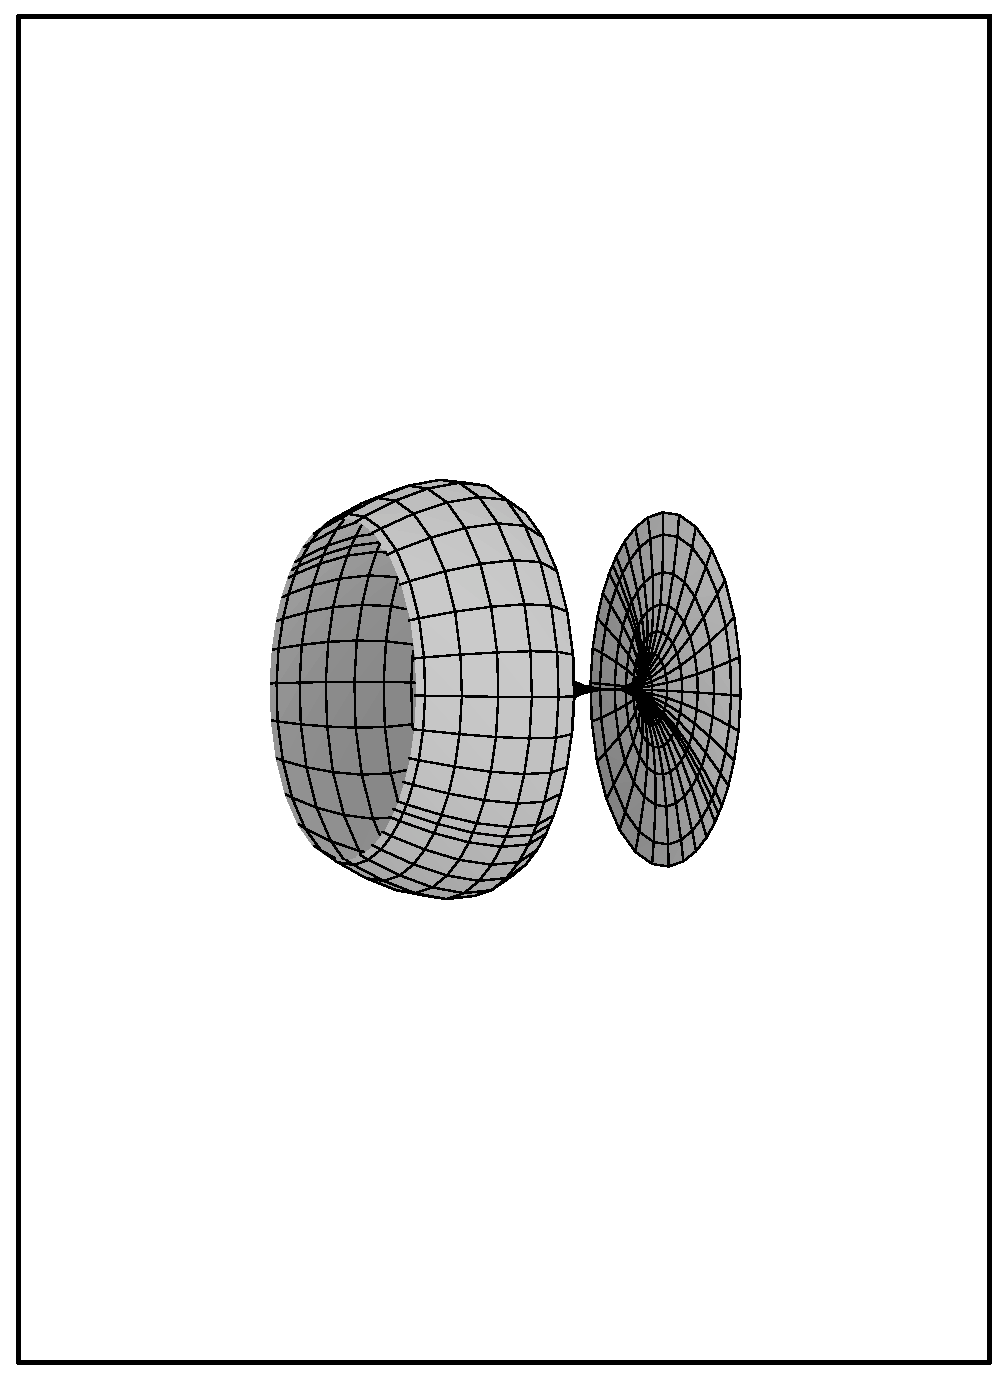
\includegraphics[angle=-90, width=0.3\textwidth]{cup2.eps}
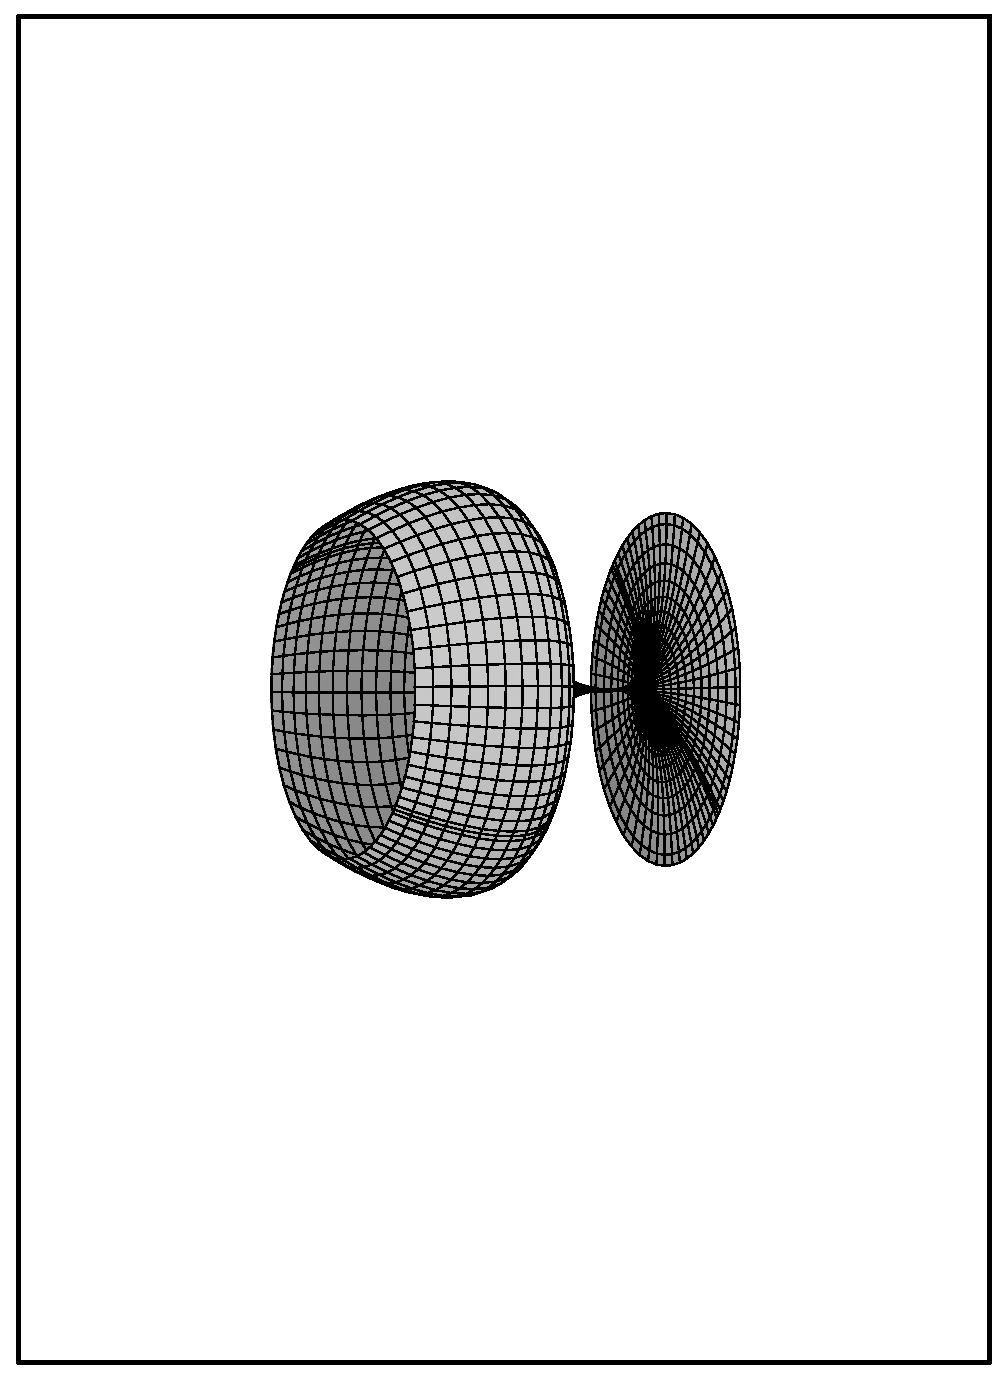
\includegraphics[angle=-90, width=0.3\textwidth]{cup3.eps}

\caption{The control polygon sequences of a cup-like rotation}
\label{fig:levfig}
\end{figure}

You can then cite them in your article as following: Fig.
\ref{fig:levfig} shows a process of level set based segmentation.



\section{Citing a Reference}
You can cite a reference by making use of the command ``\verb|\cite|" after you have labelled a bibliography\cite{labelbib}.
An illustration of \TeX/\LaTeX in given in \cite{texbook}.
Please refer to \cite{NumeApp,UncaliEu,SpaceDeform,Deformation} to get a detailed format of references.
The citation in the former sentence can be made by using the command ``\verb|\cite{|\verb|NumeApp|, \verb|UncaliEu|, \verb|SpaceDeform|, \verb|Deformation}|", where NumApp, UncaliEu, etc., are user defined labels for references.
% appendix sections are done as normal sections

\section*{Acknowledgement}
Acknowledge here.
\section*{Appendix} Appendix here.
\begin{thebibliography}{00}\label{ref:ref}

% \bibitem{label}
% Text of bibliographic item

% notes:
% \bibitem{label} \note

% subbibitems:
% \begin{subbibitems}{label}
% \bibitem{label1}
% \bibitem{label2}
% If there is a note, it should come last:
% \bibitem{label3} \note
% \end{subbibitems}

\bibitem{labelbib} Bibliography, For further detail, please visit our
website, http://www.joics.com, 2004
\bibitem{NumeApp} R. H. Wang, {\it Numerical Approximation}, Higher Education Press, Beijing, 1999
\bibitem{UncaliEu} A. Fusiello, Uncalibrated euclidean reconstruction: a review, Image and Vision Computing 18 (2000) 555-563
\bibitem{Deformation} X. Provot, Deformation constraints in a mass-spring model to describe rigid cloth behavior, in: Proc. Graphics Interface '95, 1995, pp. 147-154
\bibitem{SpaceDeform} Y. Sun, Space Deformation with Geometric Constraint, M. S. Thesis, Department of Applied Mathematics, Dalian University of Technology, March 2002
\bibitem{texbook} Donald E. Knuth, {\it The TEXbook}, Addison--Welsey, 1996
\bibitem{canonical}E. L. Ortiz, Canonical polynomials in the Lanczos tau-method, in: B. Scaife (Ed.), Studies in Numerical Analysis, Academic Press, New York, 1974, pp. 73-93
\end{thebibliography}

\end{document}
